\chapter{LHCb}
The Large Hadron Collider (LHC) is a particle accelerator at CERN, the European
organization for nuclear research, close to Geneva and LHCb is one of the four main experiments at the LHC. The data used in this analysis was taken during Run 1 of the pp collision with 7 TeV center-of-mass energy but filtered through different triggering techniques. The schematic diagram of the LHCb is shown in Figure \ref{LHCb}.\\

\begin{figure}[H]
    \centering
    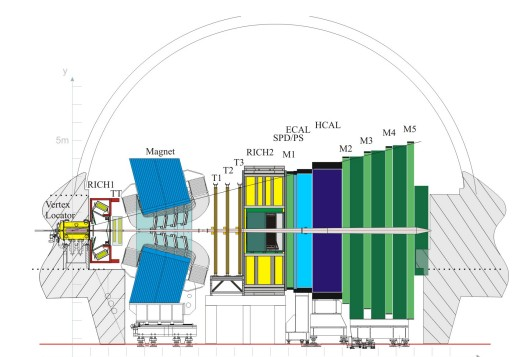
\includegraphics[width=0.8\linewidth]{Figure/LHCb.jpg}
    \caption{Schematic diagram of the LHCb detector.}
    \label{LHCb}
\end{figure}

Unlike the large, symmetric detectors like ATLAS and CMS, LHCb has a forward geometry, focusing on particles emitted at small angles relative to the beam line, where b-hadrons are most frequently produced. The detector is a forward spectrometer, about 20 meters long, consisting of several specialized components arranged in a sequence. Closest to the collision point is the Vertex Locator (VELO), which uses high-precision silicon sensors to detect where particles originate and helps distinguish the decay vertices of short-lived particles. Following VELO is the tracking system, which measures the momentum of charged particles as they curve in a magnetic field provided by a large dipole magnet.\\

To identify the type of each particle, LHCb uses two RICH (Ring Imaging Cherenkov) detectors that detect light emitted when charged particles travel faster than the speed of light in a medium. These detectors help distinguish between similar particles like pions, kaons, and protons. Further along the detector are the electromagnetic and hadronic calorimeters, which measure the energy of electrons, photons, and hadrons by absorbing them. At the far end is the muon detection system, which identifies muons that pass through all other layers of the detector, as muons are crucial in identifying many rare decay processes. LHCb also features a sophisticated trigger system, which quickly filters out the vast majority of uninteresting collisions and keeps only the events likely to contain b-hadrons or other particles of interest. The combination of precision vertex detection, excellent momentum measurement, and robust particle identification makes LHCb exceptionally capable of studying rare decays, CP violation, and potential signs of new physics beyond the Standard Model. Two of the key uses of the LHCb detector is to study of matter-antimatter asymmetry and rare decays of b- and c-quarks.\\
